\section{Passo 8 — Harmonizar depositantes e inventores}
\label{sec:passo8}

\subsection*{Objetivo}
Transformar nomes exportados (grafias diferentes, subsidiárias, traduções) em identificadores
consistentes, para que a contagem por depositante faça sentido.

\begin{figure}[H]
\centering
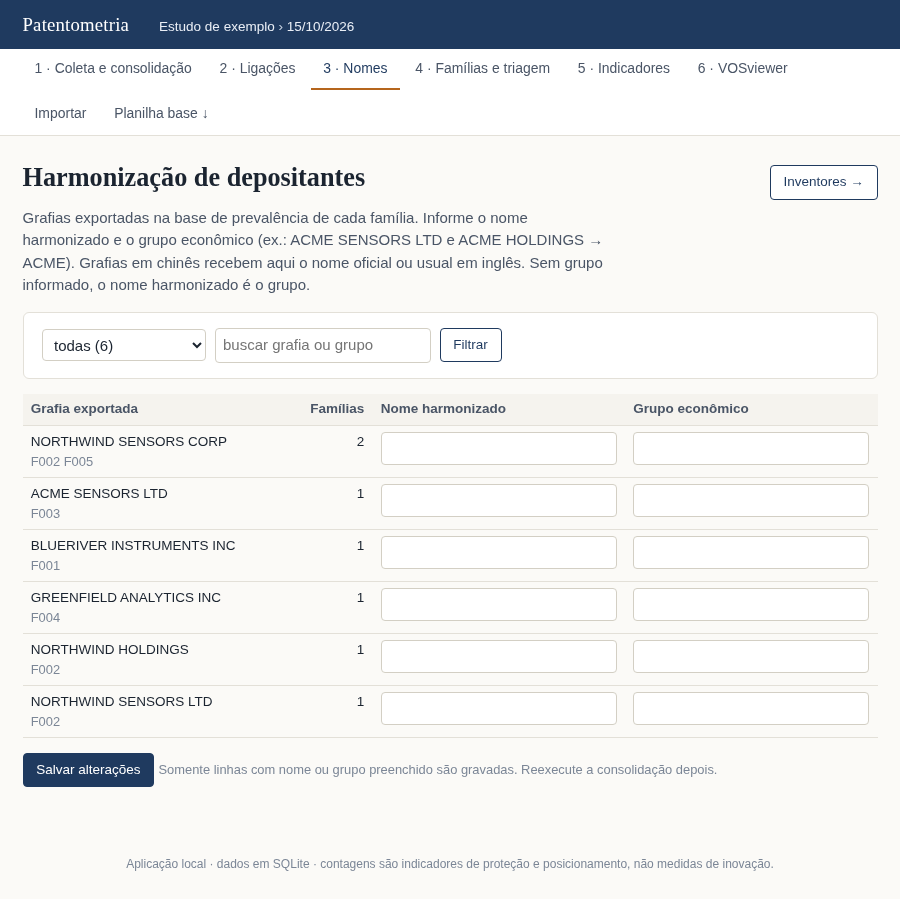
\includegraphics[width=0.72\linewidth]{img/10_depositantes.png}
\caption{Harmonização de depositantes: cada grafia exportada aparece com o número de famílias, um
campo de nome harmonizado e um campo de grupo econômico.}
\label{fig:depositantes}
\end{figure}

\subsection*{O que fazer}
\begin{enumerate}
\item Abra \textbf{Nomes} e escolha \textbf{Depositantes}.
\item Para cada grafia, preencha o \textbf{nome harmonizado} (a forma que você vai citar) e o
      \textbf{grupo econômico}, quando houver controladora comum.
\item Use o filtro para trabalhar por família de grafias.
\item Clique em \textbf{Salvar alterações} e reconsolide a rodada.
\item Repita em \textbf{Inventores}, com atenção a abreviações e homônimos.
\end{enumerate}

\subsection*{Como interpretar}
A tela separa três conceitos que costumam ser confundidos:

\begin{itemize}
\item \textbf{Grafia exportada}: o que a base entregou, sem tratamento.
\item \textbf{Nome harmonizado}: a forma única usada nas tabelas e nos textos.
\item \textbf{Grupo econômico}: a controladora que reúne várias pessoas jurídicas.
\end{itemize}

O número ao lado da grafia é o de \emph{famílias} em que ela aparece. Depois da harmonização, o
indicador de concentração passa a somar famílias por grupo, e não por grafia --- é isso que evita
concluir que um mercado é fragmentado quando, na verdade, são três subsidiárias do mesmo grupo.

\begin{nota}[Atribuições, não famílias]
Uma família com dois depositantes conta para os dois. Por isso a soma das colunas pode ser maior que o
número de famílias. A tela de indicadores informa o total de atribuições justamente para tornar essa
diferença visível.
\end{nota}

\begin{alerta}[Erro comum]
Preencher grupo econômico sem nome harmonizado. A aplicação só grava linhas com nome ou grupo
preenchido; sem harmonização, a grafia original continua sendo a unidade de contagem.
\end{alerta}

\subsection*{Checkpoint}
\marcador\; As grafias relevantes têm nome harmonizado, os grupos estão preenchidos e os indicadores, após
reconsolidar, mostram menos depositantes do que grafias.
